\documentclass[11pt,a4paper,openany]{report}

\usepackage[spanish,es-nodecimaldot]{babel}
\usepackage[a4paper,margin=2.3cm,headheight=15pt]{geometry}
\usepackage{microtype}
\usepackage{booktabs}
\usepackage{longtable}
\usepackage{tabularx}
\usepackage{array}
\usepackage{enumitem}
\usepackage{xcolor}
\usepackage{tikz}
\usetikzlibrary{arrows.meta,positioning,fit,backgrounds,shapes.geometric}
\usepackage{listings}
\usepackage{fancyhdr}
\usepackage{hyperref}
\usepackage{graphicx}

\definecolor{ink}{HTML}{10231E}
\definecolor{leaf}{HTML}{1FAF78}
\definecolor{gold}{HTML}{D6A93B}
\definecolor{soft}{HTML}{EEF5F1}
\definecolor{warn}{HTML}{D65A3A}
\definecolor{codebg}{HTML}{F5F7F6}

\hypersetup{
  colorlinks=true,
  linkcolor=ink,
  urlcolor=leaf,
  citecolor=gold,
  pdftitle={Informe final - Radar Electoral Big Data},
  pdfauthor={Sixto Caceres Terrones}
}

\pagestyle{fancy}
\fancyhf{}
\fancyhead[L]{Radar Electoral Big Data}
\fancyhead[R]{Informe técnico}
\fancyfoot[C]{\thepage}

\setlist[itemize]{topsep=3pt,itemsep=2pt}
\setlist[enumerate]{topsep=3pt,itemsep=2pt}
\renewcommand{\arraystretch}{1.18}

\lstset{
  basicstyle=\ttfamily\small,
  backgroundcolor=\color{codebg},
  frame=single,
  rulecolor=\color{leaf!35},
  breaklines=true,
  columns=fullflexible,
  keepspaces=true,
  showstringspaces=false,
  keywordstyle=\color{leaf!70!black},
  commentstyle=\color{gray}
}

\newcommand{\topic}[1]{\texttt{#1}}
\newcommand{\statusok}{\textcolor{leaf}{\textbf{conectado}}}
\newcolumntype{Y}{>{\raggedright\arraybackslash}X}

\begin{document}

\begin{titlepage}
  \color{ink}
  \vspace*{2.2cm}
  {\Large\textcolor{gold!80!black}{PROYECTO BIG DATA}\par}
  \vspace{0.6cm}
  {\Huge\bfseries Radar electoral de\\[0.2cm]comentarios en vivo\par}
  \vspace{0.7cm}
  {\LARGE Informe de arquitectura, procesamiento NLP\\[0.15cm]y operación distribuida\par}
  \vfill
  \begin{tabular}{@{}ll@{}}
    Alumno & Sixto Caceres Terrones\\
    Plataforma & AWS EMR, S3, Kafka, Flink y Spark\\
    Interfaz & Dashboard web local\\
    Repositorio & \url{https://github.com/LaterSpec/bigdata-spark-flink}\\
    Fecha & 30 de junio de 2026\\
    Versión & Arquitectura distribuida vigente
  \end{tabular}
  \vspace{1.2cm}
\end{titlepage}
\color{ink}

\pagenumbering{roman}
\tableofcontents
\clearpage

\chapter*{Resumen}
\addcontentsline{toc}{chapter}{Resumen}

El sistema analiza comentarios de YouTube Live Chat asociados al discurso electoral peruano. La fuente durable reside en Amazon S3; un productor Python reproduce los registros como flujo y los publica en un clúster Kafka KRaft de tres nodos. Desde el topic \topic{raw\_youtube\_chat}, cinco jobs Flink realizan análisis de baja latencia y Spark procesa rangos disjuntos de 1,000 registros. Los resultados streaming regresan a Kafka y los productos batch se almacenan como Parquet en S3 Curated.

La solución combina dos familias de técnicas NLP: reglas lingüísticas específicas del contexto peruano y modelos Spark ML entrenados con OffendES. Las reglas aportan señales explicables de terruqueo, fraude electoral, instituciones, actores, insultos y discriminación; el modelo aporta clasificación general de ofensividad en español. El nivel de riesgo híbrido evita interpretar la predicción ML cruda como una verdad política.

La validación distribuida registró quorum Kafka de tres voters, cero particiones offline, cinco consumidores Flink, batches Spark sin solapamiento y salidas S3 separadas por rango. El dashboard ofrece control de arranque y parada, feeds en vivo, contadores, batches y diagnóstico. Mientras existe una sesión AWS activa, el estado principal se muestra como \statusok{} con foco verde; las advertencias técnicas permanecen visibles en el panel detallado.

\clearpage
\pagenumbering{arabic}

\chapter{Arquitectura del clúster}

\section{Topología física}

La plataforma separa el bus de eventos del cómputo. Esta decisión evita que una aplicación Spark intensiva compita directamente con Kafka por memoria y CPU.

\small
\begin{longtable}{>{\raggedright\arraybackslash}p{2.0cm}>{\raggedright\arraybackslash}p{3.1cm}>{\raggedright\arraybackslash}p{3.2cm}>{\raggedright\arraybackslash}p{5.8cm}}
\toprule
\textbf{Capa} & \textbf{Nodo o clúster} & \textbf{Rol} & \textbf{Servicios}\\
\midrule
\endfirsthead
\toprule
\textbf{Capa} & \textbf{Nodo o clúster} & \textbf{Rol} & \textbf{Servicios}\\
\midrule
\endhead
Datos & Amazon S3 & Fuente durable & CSV Raw, modelos OffendES, Parquet Curated, reportes y agregados.\\
Eventos & Primary, nodo 1 & Entrada y coordinación & Broker/controller 1, producer Python, monitor, SSH y descubrimiento EMR.\\
Eventos & Core, nodo 2 & Réplica Kafka & Broker/controller 2, réplica e ISR.\\
Eventos & Core, nodo 3 & Réplica Kafka & Broker/controller 3, réplica e ISR.\\
Streaming & Primer worker & Baja latencia & Flink 1.17.1, cinco jobs, YARN y acceso privado a Kafka.\\
Batch & Workers compute & Cómputo por rangos & Spark 3.4.1 sobre YARN, launchers, locks y estados JSON atómicos.\\
Control & Máquina local & Plano de control & Node.js, API HTTP, dashboard, SSH/SCP y llave PEM local.\\
\bottomrule
\end{longtable}
\normalsize

\section{Roles y disponibilidad}

\begin{itemize}
  \item Los tres nodos Kafka combinan los roles \topic{broker,controller}. El quorum utiliza puerto 9093 y el tráfico de clientes usa 9092.
  \item Los topics operativos tienen tres particiones, factor de replicación 3 y \topic{min.insync.replicas=2}.
  \item El primary descubre dinámicamente los DNS privados de los core nodes; la llave privada no se copia a AWS.
  \item Flink usa grupos estables. Si un job cae, su offset confirmado permite medir el lag y reanudar.
  \item Spark mantiene rangos inmutables e idempotentes. La política segura es \topic{SPARK\_MAX\_CONCURRENCY=1}.
\end{itemize}

\chapter{Arquitectura detallada del pipeline}

\section{Diagrama de componentes}

\begin{figure}[htbp]
\centering
\resizebox{\textwidth}{!}{
\begin{tikzpicture}[
  x=1cm,
  y=1cm,
  box/.style={draw=ink!55, rounded corners=3pt, fill=soft, minimum height=11mm, text width=2.45cm, align=center, font=\small},
  bus/.style={draw=gold!80!black, rounded corners=3pt, fill=gold!12, minimum height=11mm, text width=2.55cm, align=center, font=\small},
  engine/.style={draw=leaf!80!black, rounded corners=3pt, fill=leaf!10, minimum height=11mm, text width=2.45cm, align=center, font=\small},
  arrow/.style={-{Latex[length=2.4mm]}, thick, draw=ink!75}
]
  \node[box] (s3raw) at (0,3) {S3 Raw\\youtube\_lake.csv};
  \node[box] (producer) at (3.1,3) {Producer Python\\fila a fila};
  \node[bus] (raw) at (6.25,3) {Kafka KRaft\\raw\_youtube\_chat};
  \node[box] (monitor) at (3.1,1) {Monitor\\quorum, tasas y lag};

  \node[engine] (flink) at (10.0,4.45) {Flink\\5 jobs streaming};
  \node[engine] (spark) at (10.0,1.55) {Spark\\batches disjuntos};

  \node[bus] (topics) at (13.2,4.45) {Resultados Flink\\y alertas};
  \node[box] (curated) at (13.2,1.55) {S3 Curated\\Parquet + reportes};
  \node[box] (dash) at (16.4,3) {Dashboard local\\control + visualización};

  \draw[arrow] (s3raw) -- (producer);
  \draw[arrow] (producer) -- (raw);
  \draw[arrow] (raw) -- (flink);
  \draw[arrow] (raw) -- (spark);
  \draw[arrow] (flink) -- (topics);
  \draw[arrow] (spark) -- (curated);
  \draw[arrow] (topics) -- (dash.north west);
  \draw[arrow] (curated) -- (dash.south west);
  \draw[arrow,dashed] (raw.south west) -- (monitor.north east);
  \draw[arrow,dashed] (monitor.south) -- ++(0,-0.65) -| (dash.south);

  \begin{scope}[on background layer]
    \node[draw=gold!60, rounded corners=5pt, fit=(producer)(raw)(monitor), inner xsep=3mm, inner ysep=6mm,
      label={[font=\bfseries\small]above:EMR\_PRIMARY}] {};
    \node[draw=leaf!60, rounded corners=5pt, fit=(flink)(spark), inner xsep=3mm, inner ysep=6mm,
      label={[font=\bfseries\small]above:EMR\_WORKERS}] {};
  \end{scope}
\end{tikzpicture}}
\caption{Pipeline distribuido vigente. Flink y Spark son consumidores independientes del mismo topic RAW.}
\end{figure}

\section{Flujo de una sesión}

\begin{enumerate}
  \item El operador inicia el dashboard y pulsa \textbf{Conectar AWS}.
  \item El bootstrap descubre tres nodos Kafka, prepara KRaft y crea los topics.
  \item El producer lee el CSV de S3, añade \topic{event\_id} y \topic{row\_number}, y publica en Kafka.
  \item Flink procesa continuamente y confirma offsets por grupo.
  \item Al existir un múltiplo completo de 1,000 eventos, Spark agenda el rango siguiente.
  \item Spark valida el tamaño exacto, aplica reglas, ML e híbrido, y escribe rutas exclusivas en S3.
  \item El dashboard consulta deltas y salud sin consumir ni modificar los offsets de los jobs.
\end{enumerate}

\section{Topics y contratos}

\begin{tabularx}{\textwidth}{p{3.7cm}p{3.1cm}Y}
\toprule
\textbf{Topic} & \textbf{Productor} & \textbf{Contenido}\\
\midrule
\topic{raw\_youtube\_chat} & Producer Python & Comentario original, metadatos de origen, número de fila y timestamp de ingestión.\\
\topic{nlp\_stream\_results} & Flink 1--4 & Normalización, métricas por ventana, señales políticas y polarización por actor.\\
\topic{alerts\_polarization} & Flink 5 & Alertas explicables con tipo, severidad, actor, reglas y puntaje local.\\
\topic{nlp\_batch\_results} & Reservado & Integración batch opcional; la salida vigente de Spark se conserva en S3.\\
\bottomrule
\end{tabularx}

\chapter{Instalación, configuración y arranque}

\section{Prerrequisitos}

\begin{itemize}
  \item EMR\_PRIMARY con tres instancias \topic{RUNNING}.
  \item Uno o más EMR\_WORKERS con Hadoop, Spark 3.4.1 y Flink 1.17.1.
  \item Conectividad privada entre clústeres y permisos S3.
  \item Node.js 18 o superior, PowerShell o Git Bash, SSH/SCP y AWS CLI.
  \item \topic{final.pem} y un archivo \topic{.env} local, ambos fuera de Git.
\end{itemize}

\section{Configuración}

\begin{lstlisting}
EMR_PRIMARY=ec2-primary.compute-1.amazonaws.com
EMR_WORKERS=ec2-compute-1.compute-1.amazonaws.com
DATA_SIZE=30000
SPARK_BATCH_SIZE=1000
SPARK_MAX_CONCURRENCY=1
\end{lstlisting}

\section{Arranque desde cero}

\begin{lstlisting}[language=bash]
cd emr_kafka_setup/dashboard
./start_dashboard.sh
# Windows: .\start_dashboard.ps1
\end{lstlisting}

Se abre \url{http://127.0.0.1:8787} y se pulsa \textbf{Conectar AWS}. Para un bootstrap directo y controlado:

\begin{lstlisting}[language=bash]
./scripts/bootstrap_emr_streaming.sh \
  --limit 2000 \
  --producer-delay-ms 10 \
  --reset-topics
\end{lstlisting}

\section{Validación}

\begin{lstlisting}[language=bash]
./scripts/aws_status_from_aws.sh \
  --data-size 2000 \
  --spark-batch-size 1000 \
  --spark-max-concurrency 1
./scripts/spark_status_from_aws.sh --max-concurrency 1
./scripts/pipeline_health_from_aws.sh
\end{lstlisting}

\section{Scripts después de reiniciar una sesión}

Si solo se cerró la terminal local, se vuelve a ejecutar el dashboard. Si también deben restaurarse producer, monitor y jobs, conservando topics y offsets:

\begin{lstlisting}[language=bash]
./scripts/restart_services_after_session.sh
# Windows:
.\scripts\restart_services_after_session.ps1
\end{lstlisting}

Estos wrappers invocan \topic{bootstrap\_emr\_streaming.sh --no-reset-topics}. Para empezar una sesión limpia se usa \textbf{Detener plataforma} y luego \textbf{Conectar AWS}.

\section{Parada segura}

\begin{lstlisting}[language=bash]
./scripts/stop_emr_streaming.sh
\end{lstlisting}

La parada cancela aplicaciones YARN, drivers Spark, jobs Flink, producer, monitor y brokers. No elimina el CSV, los modelos ni los productos S3.

\chapter{Datasets y fuentes}

\section{YouTube Live Chat electoral peruano}

El dataset principal contiene 160,464 comentarios deduplicados. Fue recolectado de chats públicos de YouTube asociados a transmisiones y discusión electoral peruana mediante \topic{yt-dlp}. El archivo durable es:

\begin{lstlisting}
s3://figuretibucket/data/raw/youtube/youtube_lake.csv
\end{lstlisting}

Las columnas relevantes se organizan así:

\begin{center}
\small
\begin{tabularx}{0.94\textwidth}{p{4.1cm}Y}
\toprule
\textbf{Columna} & \textbf{Uso en el pipeline}\\
\midrule
\topic{source\_file} & Archivo de chat del que proviene el registro.\\
\topic{video\_id} & Identificador de la transmisión de YouTube.\\
\topic{timestamp\_text} & Marca temporal legible dentro del chat.\\
\topic{timestamp\_usec} & Tiempo original en microsegundos.\\
\topic{video\_offset\_msec} & Posición relativa usada para agregados históricos.\\
\topic{author} & Autor público del mensaje.\\
\topic{message\_raw / message\_clean} & Texto original y versión preparada para análisis.\\
\bottomrule
\end{tabularx}
\normalsize
\end{center}

La fuente no incluye etiquetas humanas de ofensividad; por esa razón no se usa como corpus supervisado de entrenamiento.

\section{OffendES}

OffendES es el corpus externo etiquetado para investigación de lenguaje ofensivo en español. La copia de trabajo se conserva en S3:

\begin{lstlisting}
s3://figuretibucket/dataset/offendES/train.parquet
s3://figuretibucket/dataset/offendES/validation.parquet
s3://figuretibucket/dataset/offendES/test.parquet
\end{lstlisting}

Fuentes públicas: \url{https://huggingface.co/datasets/fmplaza/offendes} y el artículo \url{https://aclanthology.org/2021.ranlp-1.123/}. El mapeo binario usa etiquetas 0/1 como ofensivo y 2/3 como no ofensivo. El modelo multiclase conserva las cuatro categorías analíticas.

\section{Consideraciones éticas}

\begin{itemize}
  \item Las reglas y predicciones son señales analíticas, no juicios definitivos sobre personas.
  \item Términos étnicos, regionales o políticos requieren contexto humano.
  \item Los identificadores de usuarios no deben usarse para persecución, perfilado sensible ni decisiones automatizadas.
  \item El cambio de dominio entre OffendES y chat político peruano obliga a reportar incertidumbre.
\end{itemize}

\chapter{Técnicas NLP}

\section{Normalización streaming}

Flink selecciona \topic{message\_clean} o el mensaje raw, convierte a minúsculas, reduce espacios y conserva trazabilidad con topic, partición y offset. La normalización es deliberadamente ligera para sostener baja latencia.

\section{Reglas lingüísticas locales}

Se aplican expresiones y diccionarios multilabel para terruqueo, fraude, instituciones electorales, actores, polarización, lenguaje discriminatorio, insultos y spam. Cada activación aporta etiquetas y un \topic{local\_risk\_score}. La salida explica la razón del riesgo.

\section{Spark ML con OffendES}

El pipeline supervisado usa \topic{RegexTokenizer}, eliminación de stopwords, \topic{HashingTF}, IDF y regresión logística. Se entrenan un clasificador binario y otro multiclase. El entrenamiento es offline; la inferencia sobre cada batch carga modelos persistidos.

\section{Scoring híbrido}

La señal final combina confianza ML y reglas:

\begin{itemize}
  \item \textbf{Bajo}: no hay evidencia fuerte.
  \item \textbf{Medio}: predicción incierta o reglas moderadas.
  \item \textbf{Alto}: confianza elevada y/o combinación local de riesgo.
\end{itemize}

Este enfoque compensa la sobredetección del modelo general y la cobertura limitada de reglas puramente locales.

\chapter{Documentación de los 10 jobs}

\section{Idempotencia y control}

Cada batch usa un identificador como \topic{batch\_0001000}. El launcher conserva un lock y un estado JSON remoto. Si el estado ya existe no vuelve a escribir la salida; el reproceso requiere \topic{--force}. Antes de avanzar, el servidor verifica que todos los rangos anteriores estén \topic{done}.

\section{Cinco jobs Flink}

\small
\begin{longtable}{p{0.7cm}p{2.8cm}p{3.0cm}p{7.4cm}}
\toprule
\textbf{N.º} & \textbf{Job} & \textbf{Salida} & \textbf{Descripción}\\
\midrule
\endfirsthead
\toprule
\textbf{N.º} & \textbf{Job} & \textbf{Salida} & \textbf{Descripción}\\
\midrule
\endhead
F1 & Normalización & Resultados NLP & Un resultado principal por comentario; confirma offsets en \topic{flink-job1-normalize}.\\
F2 & Métricas por ventana & Resultados NLP & Ventanas de tiempo con volumen, autores únicos, longitud media, vacíos y spam aparente.\\
F3 & Señales políticas & Resultados NLP & Reglas de terruqueo, fraude, instituciones, política, discriminación e insultos.\\
F4 & Polarización por actor & Resultados NLP & Agrupa menciones, insultos y señales por actor en ventanas temporales.\\
F5 & Alertas de riesgo & Alertas & Emite solo casos que superan condiciones de alerta, con severidad y explicación.\\
\bottomrule
\end{longtable}

\section{Cinco jobs Spark}

\begin{longtable}{p{0.7cm}p{2.8cm}p{3.5cm}p{6.9cm}}
\toprule
\textbf{N.º} & \textbf{Job} & \textbf{Entrada/salida} & \textbf{Descripción}\\
\midrule
\endfirsthead
\toprule
\textbf{N.º} & \textbf{Job} & \textbf{Entrada/salida} & \textbf{Descripción}\\
\midrule
\endhead
S1 & Kafka Raw Ingest & Kafka $\rightarrow$ Parquet & Lee offsets y filtra \topic{row\_number} por rango; exige exactamente 1,000 filas.\\
S2 & Reglas locales & Parquet $\rightarrow$ reglas & Genera flags multilabel, score local y reporte de distribución.\\
S3 & Entrenamiento OffendES & OffendES $\rightarrow$ modelos & Entrena y persiste clasificadores binario y multiclase con Spark ML. Se ejecuta offline.\\
S4 & Inferencia OffendES & Parquet + modelos $\rightarrow$ ML & Aplica ambos modelos a comentarios Kafka y conserva probabilidades y clases.\\
S5 & Híbrido y agregados & Reglas + ML $\rightarrow$ Curated & Calcula nivel y razón de riesgo, agrega métricas y produce reportes S3.\\
\bottomrule
\end{longtable}
\normalsize

\chapter{Reporte de métricas}

\section{Validación distribuida de 2,000 eventos}

\begin{table}[htbp]
\centering
\begin{tabular}{lr}
\toprule
\textbf{Métrica} & \textbf{Resultado}\\
\midrule
Voters Kafka / leader & 3 / activo\\
Factor de réplica / minimum ISR & 3 / 2\\
Particiones under-replicated & 0\\
Particiones offline & 0\\
\topic{raw\_youtube\_chat} & 2,000\\
\topic{nlp\_stream\_results} & 4,021\\
\topic{alerts\_polarization} & 10\\
Lag total Flink & 0\\
Nodos YARN compute & 2\\
Batches Spark completos / fallidos & 2 / 0\\
Solapamiento de \topic{event\_id} entre batches & 0\\
\bottomrule
\end{tabular}
\caption{Evidencia registrada en la validación distribuida.}
\end{table}

\section{Métricas ML}

\begin{tabular}{lrr}
\toprule
\textbf{Modelo} & \textbf{Accuracy} & \textbf{Macro F1}\\
\midrule
OffendES binario & 0.838968 & 0.749030\\
OffendES multiclase & 0.771939 & 0.548677\\
\bottomrule
\end{tabular}

La inferencia ML cruda marcó 53.25\% como ofensivo en YouTube, pero 60.31\% de las predicciones se concentró en confianza 0.50--0.70. Por cambio de dominio, ese porcentaje no se adopta como conclusión final.

\section{Métricas del corpus completo}

Sobre 160,464 comentarios, las reglas registraron 4.05\% de terruqueo, 5.03\% de fraude, 4.46\% de instituciones electorales, 31.36\% de menciones políticas, 5.70\% de polarización y 3.21\% de insulto general. El score local promedio fue 0.5698, con máximo 8.

El scoring híbrido produjo:

\begin{center}
\begin{tabular}{lr}
\toprule
\textbf{Nivel} & \textbf{Porcentaje}\\
\midrule
Bajo & 52.37\%\\
Medio & 42.44\%\\
Alto & 5.19\%\\
\bottomrule
\end{tabular}
\end{center}

\section{Cadencia del dashboard}

\begin{tabularx}{\textwidth}{Yrr}
\toprule
\textbf{Dato} & \textbf{Frecuencia objetivo} & \textbf{Fuente}\\
\midrule
RAW, eventos y normalizados & 3 s & live delta\\
Estado Spark & 3 s & estados remotos\\
Inventario Kafka y threshold & 5 s & offsets Kafka\\
Salud integral & 5 s & snapshot + SSH\\
\bottomrule
\end{tabularx}

\textbf{Flink normalizados} se obtiene del offset confirmado por \topic{flink-job1-normalize}. De este modo el contador representa progreso real, queda limitado por RAW y no aumenta al recargar o volver a entregar eventos visuales.

\chapter{Interfaz gráfica funcional}

La interfaz web implementa:

\begin{itemize}
  \item arranque asíncrono, progreso y parada distribuida;
  \item chat RAW y eventos Flink en vivo;
  \item tarjetas de muestra válida, normalizados, alertas y filas Spark;
  \item búsqueda y filtros de comentarios;
  \item polarización por actor y alertas;
  \item inventario de batches y comentarios ofensivos por batch;
  \item quorum Kafka, topics, lag, YARN, workers y acciones de recuperación.
\end{itemize}

El estado principal usa tres situaciones:

\begin{enumerate}
  \item \textbf{sin conexión}: no existe sesión activa;
  \item \textbf{consultando}: se está obteniendo el primer diagnóstico;
  \item \textbf{conectado}: sesión AWS activa, texto y foco verde.
\end{enumerate}

Una condición técnica degradada no cambia el encabezado a ``desconectado'': se conserva en las acciones de diagnóstico. Si Kafka deja de responder, el último estado válido permanece visible y la plataforma nunca se reinicia automáticamente.

\chapter{Capturas del dashboard en operación}

\begingroup\sloppy\emergencystretch=2em

Este capítulo documenta la interfaz web durante una sesión activa sobre AWS. Las capturas corresponden a una corrida con más de 75\,000 comentarios ingeridos desde Kafka y tres batches Spark completados. Cada figura ilustra una capa distinta del plano de observabilidad: visión global del pipeline, streaming Flink con reglas y procesamiento batch con ML.

\section{Vista general y chat en vivo}

La primera captura muestra la pantalla principal del \emph{Radar electoral de comentarios en vivo}. En la cabecera se resume la ruta de datos
\texttt{S3 RAW $\rightarrow$ EMR\_PRIMARY / KAFKA $\rightarrow$ EMR\_WORKERS / FLINK + SPARK}
y los controles operativos: pausar la cinta de reproducción, detener la plataforma y el indicador de sesión \statusok{}.

\begin{figure}[htbp]
  \centering
  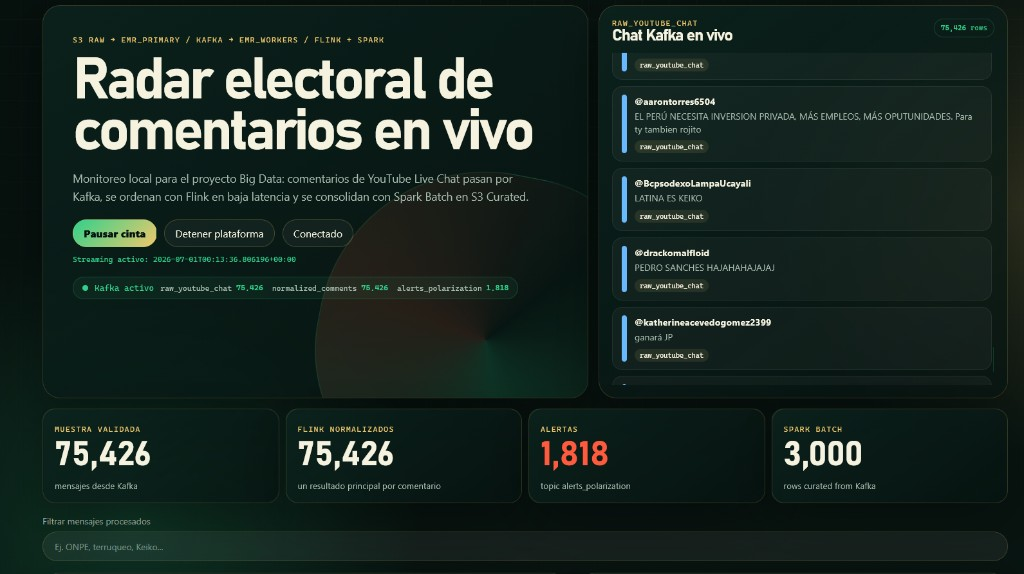
\includegraphics[width=\textwidth]{images/dashboard_vista_general.png}
  \caption{Vista general del dashboard con chat Kafka en vivo, contadores de topics y tarjetas de KPI.}
  \label{fig:dashboard-vista-general}
\end{figure}

El panel izquierdo confirma que Kafka está activo e informa los offsets acumulados de \topic{raw\_youtube\_chat} (75\,426), \topic{normalized\_comments} (75\,426) y \topic{alerts\_polarization} (1\,818). El panel derecho, titulado \emph{Chat Kafka en vivo}, despliega el feed RAW con autor y texto de cada comentario electoral peruano.

Las cuatro tarjetas inferiores sintetizan el progreso del pipeline:
\begin{itemize}
  \item \textbf{Muestra validada}: total de mensajes publicados en Kafka y visibles para Flink y Spark.
  \item \textbf{Flink normalizados}: un resultado principal por comentario, alineado con el offset confirmado del job~1.
  \item \textbf{Alertas}: eventos emitidos en \topic{alerts\_polarization} por el job Flink~5.
  \item \textbf{Spark batch}: filas ya curadas en S3 a partir de rangos disjuntos de 1\,000 eventos (3\,000 en esta sesión).
\end{itemize}

La barra inferior permite filtrar mensajes procesados por palabras clave (\emph{ONPE}, \emph{terruqueo}, \emph{Keiko}, etc.), conectando la observabilidad en tiempo real con el análisis cualitativo del corpus.

\section{Eventos Flink y comentarios filtrados por reglas}

La segunda captura divide la pantalla en dos flujos complementarios del procesamiento streaming.

\begin{figure}[htbp]
  \centering
  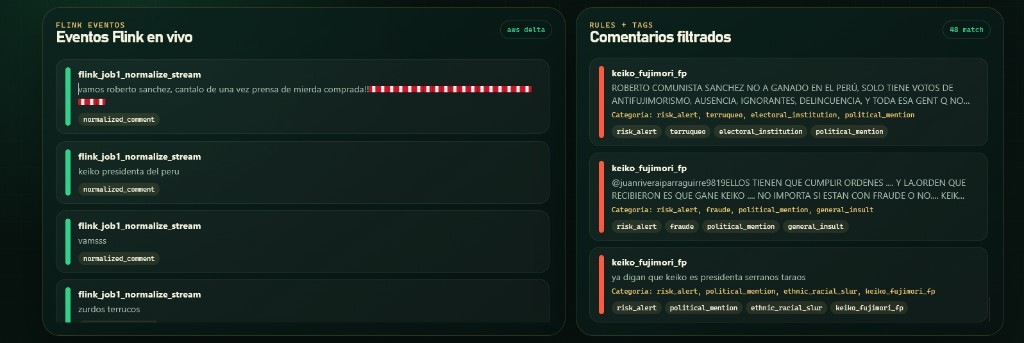
\includegraphics[width=\textwidth]{images/dashboard_flink_reglas.png}
  \caption{Panel de eventos Flink normalizados (izquierda) y comentarios filtrados por reglas y etiquetas (derecha).}
  \label{fig:dashboard-flink-reglas}
\end{figure}

En el panel \emph{Eventos Flink en vivo} (etiqueta \texttt{aws delta}) aparecen salidas del job~1 de normalización Flink. Cada tarjeta conserva el texto normalizado y la etiqueta \topic{normalized\_comment}, evidenciando la capa de ingestión de baja latencia antes de aplicar lógica política.

El panel \emph{Comentarios filtrados} (\texttt{RULES + TAGS}) muestra coincidencias del motor de reglas locales. Los registros provienen de reglas por actor (\topic{keiko\_fujimori\_fp}) y exponen categorías detectadas, entre ellas:
\begin{itemize}[nosep,topsep=2pt]
  \item alertas de riesgo (\topic{risk\_alert});
  \item menciones políticas (\topic{political\_mention});
  \item terruqueo, fraude e instituciones electorales;
  \item insultos generales y expresiones discriminatorias.
\end{itemize}
El contador \emph{48 match} resume cuántos comentarios del subconjunto visible activaron al menos una regla explicable, sin depender del modelo ML.

Esta vista demuestra la trazabilidad entre normalización streaming y señales interpretables del contexto electoral peruano.

\section{Procesamiento Spark batch y filtrado ML}

La tercera captura corresponde al módulo \emph{Spark Batch Enrichment}, donde el dashboard supervisa batches de 1\,000 eventos y la inferencia OffendES sobre cada rango completado.

\begin{figure}[htbp]
  \centering
  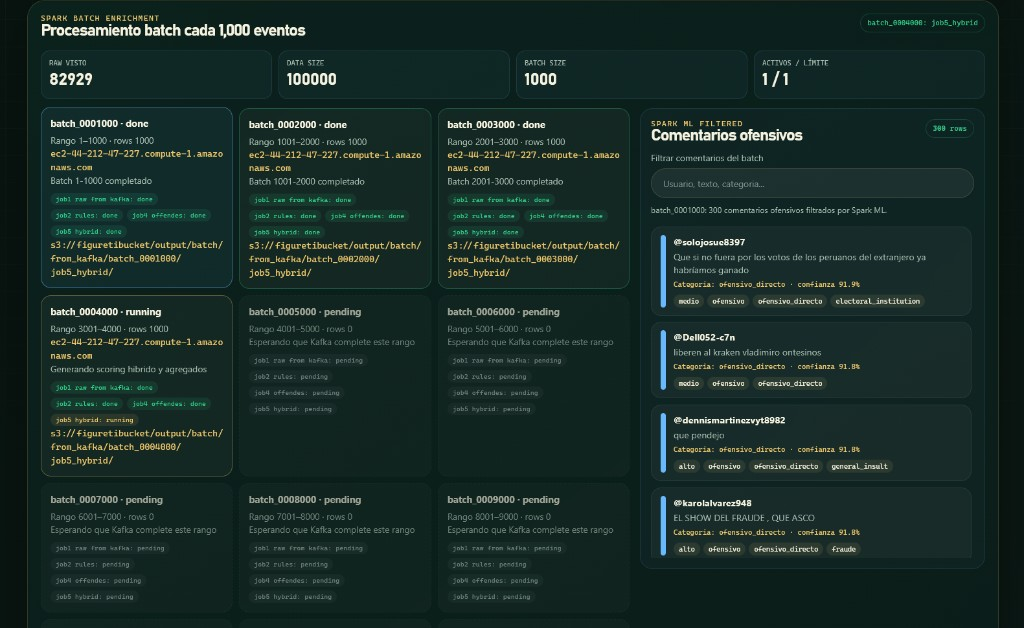
\includegraphics[width=\textwidth]{images/dashboard_spark_batch.png}
  \caption{Cuadrícula de batches Spark con sub-jobs por rango y panel lateral de comentarios ofensivos detectados por ML.}
  \label{fig:dashboard-spark-batch}
\end{figure}

La cabecera resume \textbf{RAW visto} (82\,929), \textbf{DATA SIZE} (100\,000), \textbf{BATCH SIZE} (1\,000) y \textbf{Activos / límite} (1/1), coherente con \topic{SPARK\_MAX\_CONCURRENCY=1}. La cuadrícula central muestra el ciclo de vida de cada batch:
\begin{itemize}
  \item \textbf{done} (verde): \topic{batch\_0001000} a \topic{batch\_0003000} finalizaron los cuatro sub-jobs
  (\topic{job1 raw from kafka}, \topic{job2 rules}, \topic{job4 offendes}, \topic{job5 hybrid})
  y escribieron Parquet en rutas S3 exclusivas.
  \item \textbf{running} (amarillo): \topic{batch\_0004000} ejecuta el scoring híbrido y agregados.
  \item \textbf{pending} (gris): batches posteriores esperan que Kafka complete el rango de \topic{row\_number} correspondiente.
\end{itemize}

El panel lateral \emph{Spark ML filtered: Comentarios ofensivos} lista predicciones del job~4 para \topic{batch\_0001000}: usuario, texto, categoría (\emph{ofensivo\_directo}), confianza (p.\,ej.\ 91{,}9\,\%) y etiquetas de riesgo (\emph{medio}, \emph{alto}, \emph{ofensivo}, \emph{fraude}, etc.). El resumen indica 300 comentarios ofensivos filtrados en ese batch, ilustrando cómo el dashboard cruza progreso operativo batch con evidencia cualitativa del modelo supervisado.

\endgroup

\chapter{Conclusiones}

\begin{enumerate}
  \item La separación entre Kafka y compute mejora el aislamiento de recursos y permite escalar el procesamiento sin comprometer el bus.
  \item Los grupos Flink estables y los rangos Spark disjuntos proporcionan trazabilidad reproducible desde Kafka hasta S3.
  \item El modelo OffendES aporta capacidad supervisada, pero el cambio de dominio impide usar su salida cruda como conclusión política.
  \item Las reglas locales hacen explícitas las señales peruanas; el scoring híbrido ofrece una interpretación más defendible.
  \item La operación requiere parada confirmada y concurrencia Spark controlada. La idempotencia evita relanzamientos por recargas del navegador.
  \item El dashboard ya es funcional como plano de control y observabilidad. El contador normalizado se basa ahora en offsets confirmados, no en mensajes visuales repetidos.
\end{enumerate}

\section*{Limitaciones y trabajo futuro}

\begin{itemize}
  \item Incorporar anotación humana peruana para medir precisión local y sesgo.
  \item Separar modelos de toxicidad, odio, ofensividad y polarización.
  \item Persistir series de latencia extremo a extremo para percentiles p50/p95/p99.
  \item Automatizar creación y terminación de clústeres con infraestructura como código.
  \item Añadir autenticación al plano de control si deja de ser exclusivamente local.
\end{itemize}

\appendix
\chapter{Trazabilidad documental}

\begingroup\sloppy\emergencystretch=2em

La arquitectura vigente se documenta en el repositorio público
\url{https://github.com/LaterSpec/bigdata-spark-flink}.

Los manuales operativos principales son \topic{README.md}, \topic{architecture.md}, \topic{README\_AWS\_SETUP.md} y \topic{docs/comandos\_levantar\_desde\_cero.md}, además de los documentos en \topic{emr\_kafka\_setup/docs}.

\endgroup

\chapter{Rutas principales}

\begin{lstlisting}
emr_kafka_setup/dashboard/server.js
emr_kafka_setup/dashboard/app.js
emr_kafka_setup/dashboard/scripts/bootstrap_emr_streaming.sh
emr_kafka_setup/dashboard/scripts/stop_emr_streaming.sh
emr_kafka_setup/flink/jobs/FlinkKafkaStreamingJobs.java
emr_kafka_setup/spark/jobs/
doc/informe_final.tex
\end{lstlisting}

\end{document}
